\section{Using Existing EMF Projects in eMoflon}
\label{sec : Ecore2GenModel}
	
This chapter contains stepwise instructions on how to use existing \mbox{EMF}/\-Ecore projects with an eMoflon project. 
As an example, we shall implement a small subset of the \texttt{Ecore -> GenModel} transformation. 
The \emph{GenModel} for a given Ecore model can be viewed as a \emph{wrapper} that contains additional Java code generation specific details.
These details are separated from the Ecore model to keep it free of such ``low-level'' information and settings.

As the metamodel for \textsf{GenModels} is part of the EMF/Ecore standard, this is an example of an existing metamodel which must be integrated in eMoflon before you can, for example, specify the transformation using SDMs. 
Based on this example, the basic workflow for using an existing EMF project in eMoflon is described in the following.

\subsection{Modelling relevant aspects in EA}
\label{sec: Set Up the Example}

The first step is to get the existing metamodel into EA.
A complete and automatic import of existing Ecore files in EA is currently not possible and, therefore, \emph{relevant parts} of the existing metamodel (\texttt{GenModel}) have to be modelled manually in EA.
Although this might sound frightening (especially for large complex metamodels), the emphasis here on \emph{relevant} indicates that only elements that are used for the transformation have to be present in EA and can be added iteratively as the transformation grows.

\begin{enumerate}
\item[$\blacktriangleright$] To specify our example transformation, create a new metamodel project \texttt{EcoreToGenModel} in Eclipse, check the option \texttt{Add eMoflon languages} in the wizard, and switch to EA by double-clicking the created \texttt{Ecore\-To\-Gen\-Model.eap} file.
\item[$\blacktriangleright$] Note the packages already present in EA (eMoflon Languages), especially \textsf{Ecore}, which we shall use for the transformation.
\item[$\blacktriangleright$] Create a new package \texttt{GenModel} and model the elements as depicted in Fig.~\ref{fig_gMM}.
The actual \texttt{GenModel} metamodel contains lots more elements, but this subset is sufficient for our task.
\end{enumerate}
\begin{figure}[htbp]
\begin{center}  
	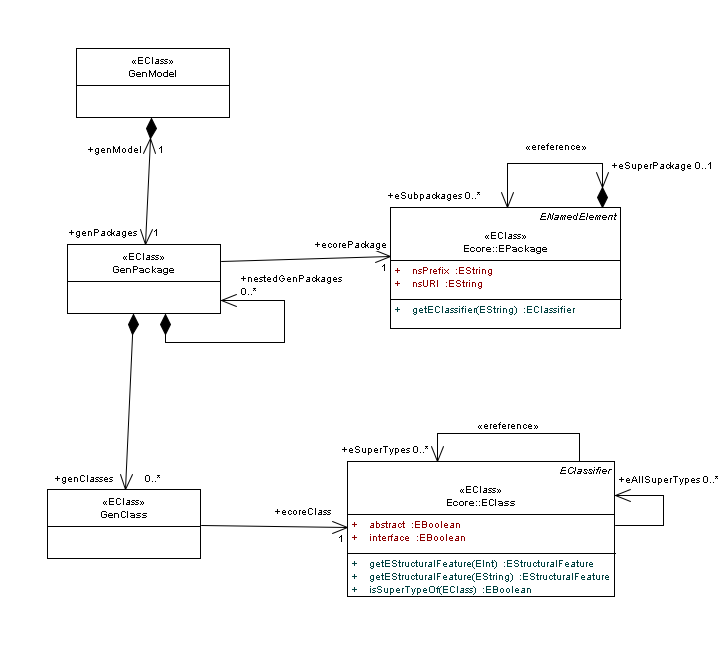
\includegraphics[width=1.0\textwidth]{pics/Ecore2GenModel_Bilder/EA_genMETAmodel.png}
	\caption{MetaModel of GenModel}  
\label{fig_gMM}
\end{center}
\end{figure} 

\begin{enumerate}  
\item[$\blacktriangleright$] Create another package \texttt{Ecore2GenModel} to contain the \texttt{Transformer} class with the methods as depicted in Fig.~\ref{fig_e2gm}.
\item[$\blacktriangleright$] Implement the SDMs depicted in Figs.~\ref{fig_pack2gm} and \ref{fig_transf}.
\end{enumerate}

\begin{figure}[htbp]
\begin{center}  
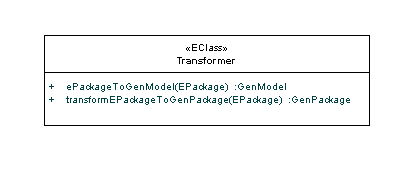
\includegraphics[width=0.8\textwidth]{pics/Ecore2GenModel_Bilder/EA_ecore2gM.png}
\caption{Methods in \textsf{Transformer}}  
\label{fig_e2gm}
\end{center}
\end{figure} 

\begin{figure}[htbp]
\begin{center}  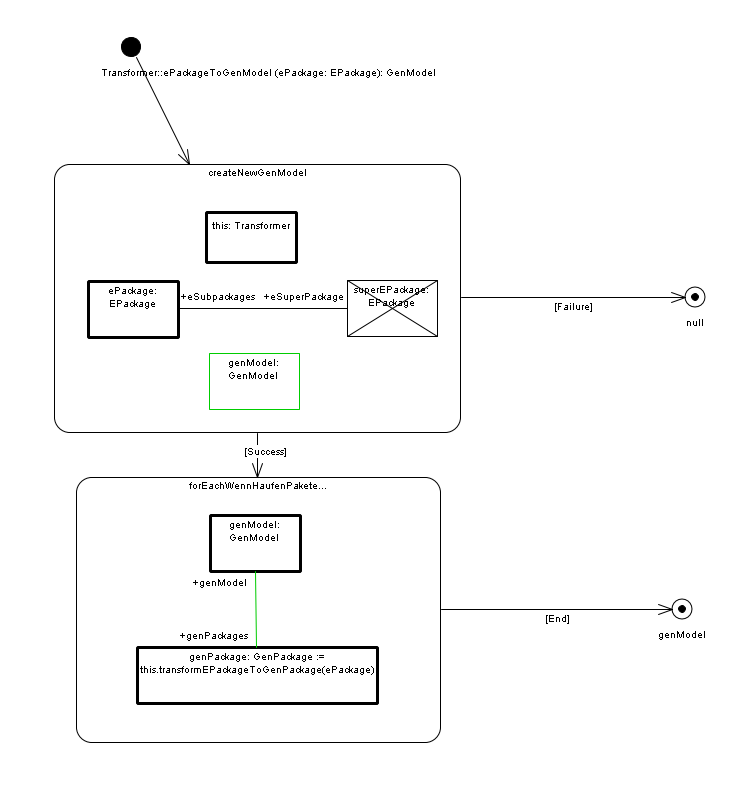
\includegraphics[width=1.0\textwidth]{pics/Ecore2GenModel_Bilder/EA_ePack2gM.png}
        \caption{Main method for \textsf{EPackage} to \textsf{GenModel} transformation}  
  \label{fig_pack2gm}
\end{center}
\end{figure} 

\begin{figure}[htbp]
\begin{center}  
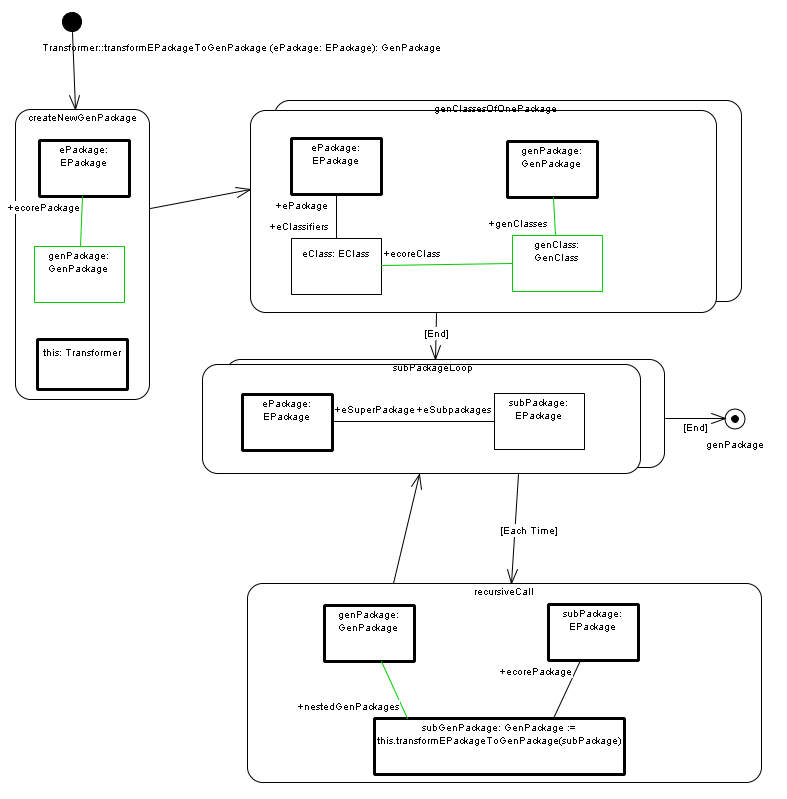
\includegraphics[width=1.0\textwidth]{pics/Ecore2GenModel_Bilder/EA_transPack2gM.png}
\caption{Helper function to transform all \textsf{EPackages} to \textsf{GenPackages}}  
\label{fig_transf}
\end{center}
\end{figure} 


\subsection{Configuration for code generation in Eclipse}
\label{sec:Project Combination}

As there is already generated code (provided via a plugin in Eclipse) for the existing \textsf{GenModel} metamodel, we do \emph{not} want to export our incomplete subset of \textsf{GenModel} in EA. 
\begin{enumerate}
\item[$\blacktriangleright$] To prevent this, right-click the \textsf{GenModel} package in EA and select ``Properties/Moflon'' and change the tagged value \texttt{Moflon::Export} to \texttt{false} (Fig.~\ref{fig_customNS}).
\end{enumerate}

Furthermore, we have to set the ``real'' name and URI of the project to be used in Eclipse so that references are exported properly. 
\begin{enumerate}
\item[$\blacktriangleright$] In the ``Properties/Moflon" dialogue for \textsf{GenModel}, create the new tagged values \texttt{Moflon::CustomNsPrefix} and \texttt{Moflon::CustomNsUri} and set them according to Fig.~\ref{fig_customNS}.
These values can be determined by inspecting the corresponding values in the existing .ecore file (i.e.,~the existing metamodel).
\end{enumerate}

\begin{figure}[htbp]
\begin{center}  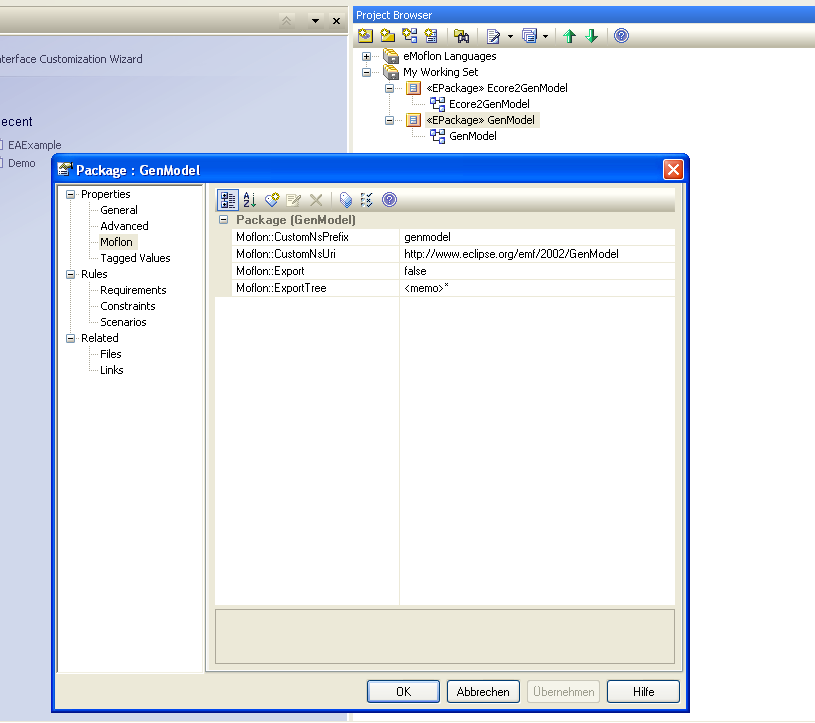
\includegraphics[width=0.87\textwidth]{pics/Ecore2GenModel_Bilder/8_nsUriPre.png}
  \caption{}  
  \label{fig_customNS}
\end{center}
\end{figure}

\begin{enumerate}
\item[$\blacktriangleright$] Export all projects as usual to your Eclipse workspace and update the metamodel project by pressing \textsf{F5}.
\item[$\blacktriangleright$] Convert the generated Eclipse project \texttt{Ecore2GenModel} to a \emph{plugin project} by right-clicking the project and selecting ``Configure/Convert to Plug-in Projects...''.
This makes it easier to set the required dependencies for code generation.
\item[$\blacktriangleright$] Now right-click \texttt{Ecore2GenModel} and choose ``Plug-in Tools/Open Manifest''.
In the window that opens up, choose the \texttt{Dependencies} tab, click \texttt{Add}, and type in \texttt{org.eclipse.emf.codegen.ecore} (which includes both the \textsf{Ecore} and \textsf{GenModel} libraries as required).
\end{enumerate}

Although we have already specified the name and URI of the existing project (in our case \textsf{GenModel}) in EA, we now have to tell eMoflon where to find the implementation (generated code) for the existing project. 
\begin{enumerate}
\item[$\blacktriangleright$] Open the \texttt{moflon.properties} file located in your project folder and insert the following lines:\\
\texttt{{\tiny ADDITIONAL\_DEPENDENCIES=platform:/plugin/org.eclipse.emf.codegen.ecore/model/GenModel.ecore}}\\
\texttt{{\tiny ADDITIONAL\_USED\_GEN\_PACKAGES=platform:/plugin/org.eclipse.emf.codegen.ecore/model/GenModel.genmodel}}
\end{enumerate}

Finally, to compensate for some cases where our naming conventions were violated, add the following mappings as corrections:

\begin{enumerate}
\item[$\blacktriangleright$] An \emph{import mapping} for correct generation of the required import:\\
\texttt{\tiny IMPORT\_MAPPINGS=genmodel-> org.eclipse.emf.codegen.ecore.genmodel}
\item [$\blacktriangleright$] A \emph{factory mapping} to ensure that \texttt{GenModelFactory} is used as the factory for creating elements in the transformation instead of \texttt{Genmodel\-Factory}, which would be the default convention:\\
\texttt{\tiny FACTORY\_MAPPING=genmodel-> GenModelFactory}
\end{enumerate}

Your \textsf{moflon.properties} file should now closely resemble Fig.~\ref{fig_mofProp}.
Now generate code once more for the project and ensure with a JUnit test that the transformation behaves as expected.

\begin{figure}[htbp]
\begin{center}  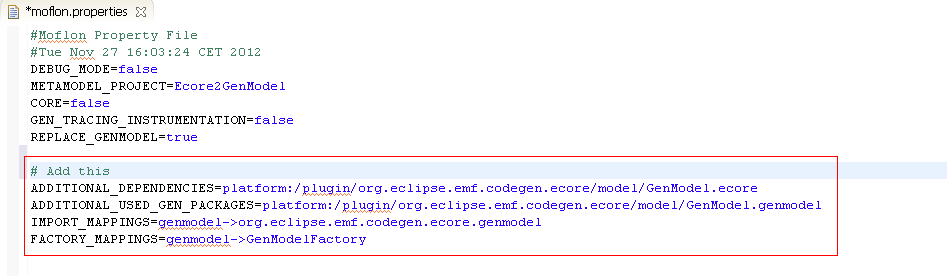
\includegraphics[width=1.3\textwidth]{pics/Ecore2GenModel_Bilder/9_mofProperties.png}
  \caption{Additional properties for code generation}  
  \label{fig_mofProp}
\end{center}
\end{figure}  







